\documentclass[10pt, a4paper]{article}

\usepackage[english]{babel}
\usepackage[utf8]{inputenc}
\usepackage{float}
\usepackage[]{amsmath} 
\usepackage{graphicx}

% Define question and answer command
\newcounter{qcounter}
\newcommand{\q}[2]
{
    \textbf{Task \refstepcounter{qcounter} \arabic{qcounter}} \\
    #2
    \par
    \vspace{0.5cm}
} 

\begin{document}

\begin{titlepage}
\centering
{
 \scshape \LARGE 
EL2450 Homework 1
}
\vfill
Andreas Froderberg - 19880730-4577
\par
Martin Favre - 19920130-0010
\end{titlepage}


\q %1
{
    A gain named Tap exists in the Tank 1 model, what is its function?
}
{
    The gain Tap models the bypass tap from the upper tank to the main tank. 
    The value 0 means that it is currently closed. A value of 1 means fully opened.
}
\q  %2
{
    Edit \textit{pid\_design.m} and fill in the transfer functions for the upper
    and lower tank.
}
{
    The figure below shows the result.
    \begin{figure}[H]
        \centering
        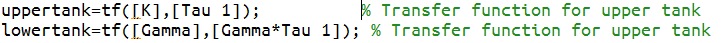
\includegraphics[width=\textwidth]{../images/q2_tfs.png}
    \end{figure}
}
\q %3
{
    What does the reference signal look like?
}
{
    The signal starts at 40 and recieves a step by 10 at 100 s which sets it to
    50.
}
\q %4
{
    Use the parameter generator to get values and fill in the transfer function
    $F$.
}
{
    Done.
}
\q %5
{
    Use the parameters to get different responses. Which is best?
}
{
    The input parameters and their respecitve system parameters are:
    \begin{table}[H]
        \centering
        \caption{Parameter values and performance.}
        \label{tab:pvals}
        \begin{tabular}{|c|c|c|c|c|c|}
            \hline
            $\chi$ & $\zeta$ & $\omega_0$ & $T_r$ [s] & $M [\%]$ & $T_s$ [s] \\
            \hline
            0.5 & 0.7 & 0.1 & 6.38 & 6.67 & 38.1 \\
            \hline
            0.5 & 0.7 & 0.2 & 3.31 & 22.6 & 18.8 \\
            \hline
            0.5 & 0.8 & 0.2 & 3.19 & 20.9 & 18.4 \\
            \hline
        \end{tabular}
    \end{table}
    The last parameter configuration works best. It is the fastest and even though 
    it has quite significant overshoot, it is still within the given tolerance
    and is thus acceptable.
}
\q %6
{
    What is the cutoff frequency for the open loop system? How was this derived?
}
{
    The open loop system is $G_o=FG$ and the cutoff frequency is the
    frequency when the amplitude gain is 0 dB. Using the bode plots this
    frequency is found to be around $\omega_c=0.35 \text{rad/s}$, see figure
    below.
    \begin{figure}[H]
        \centering
        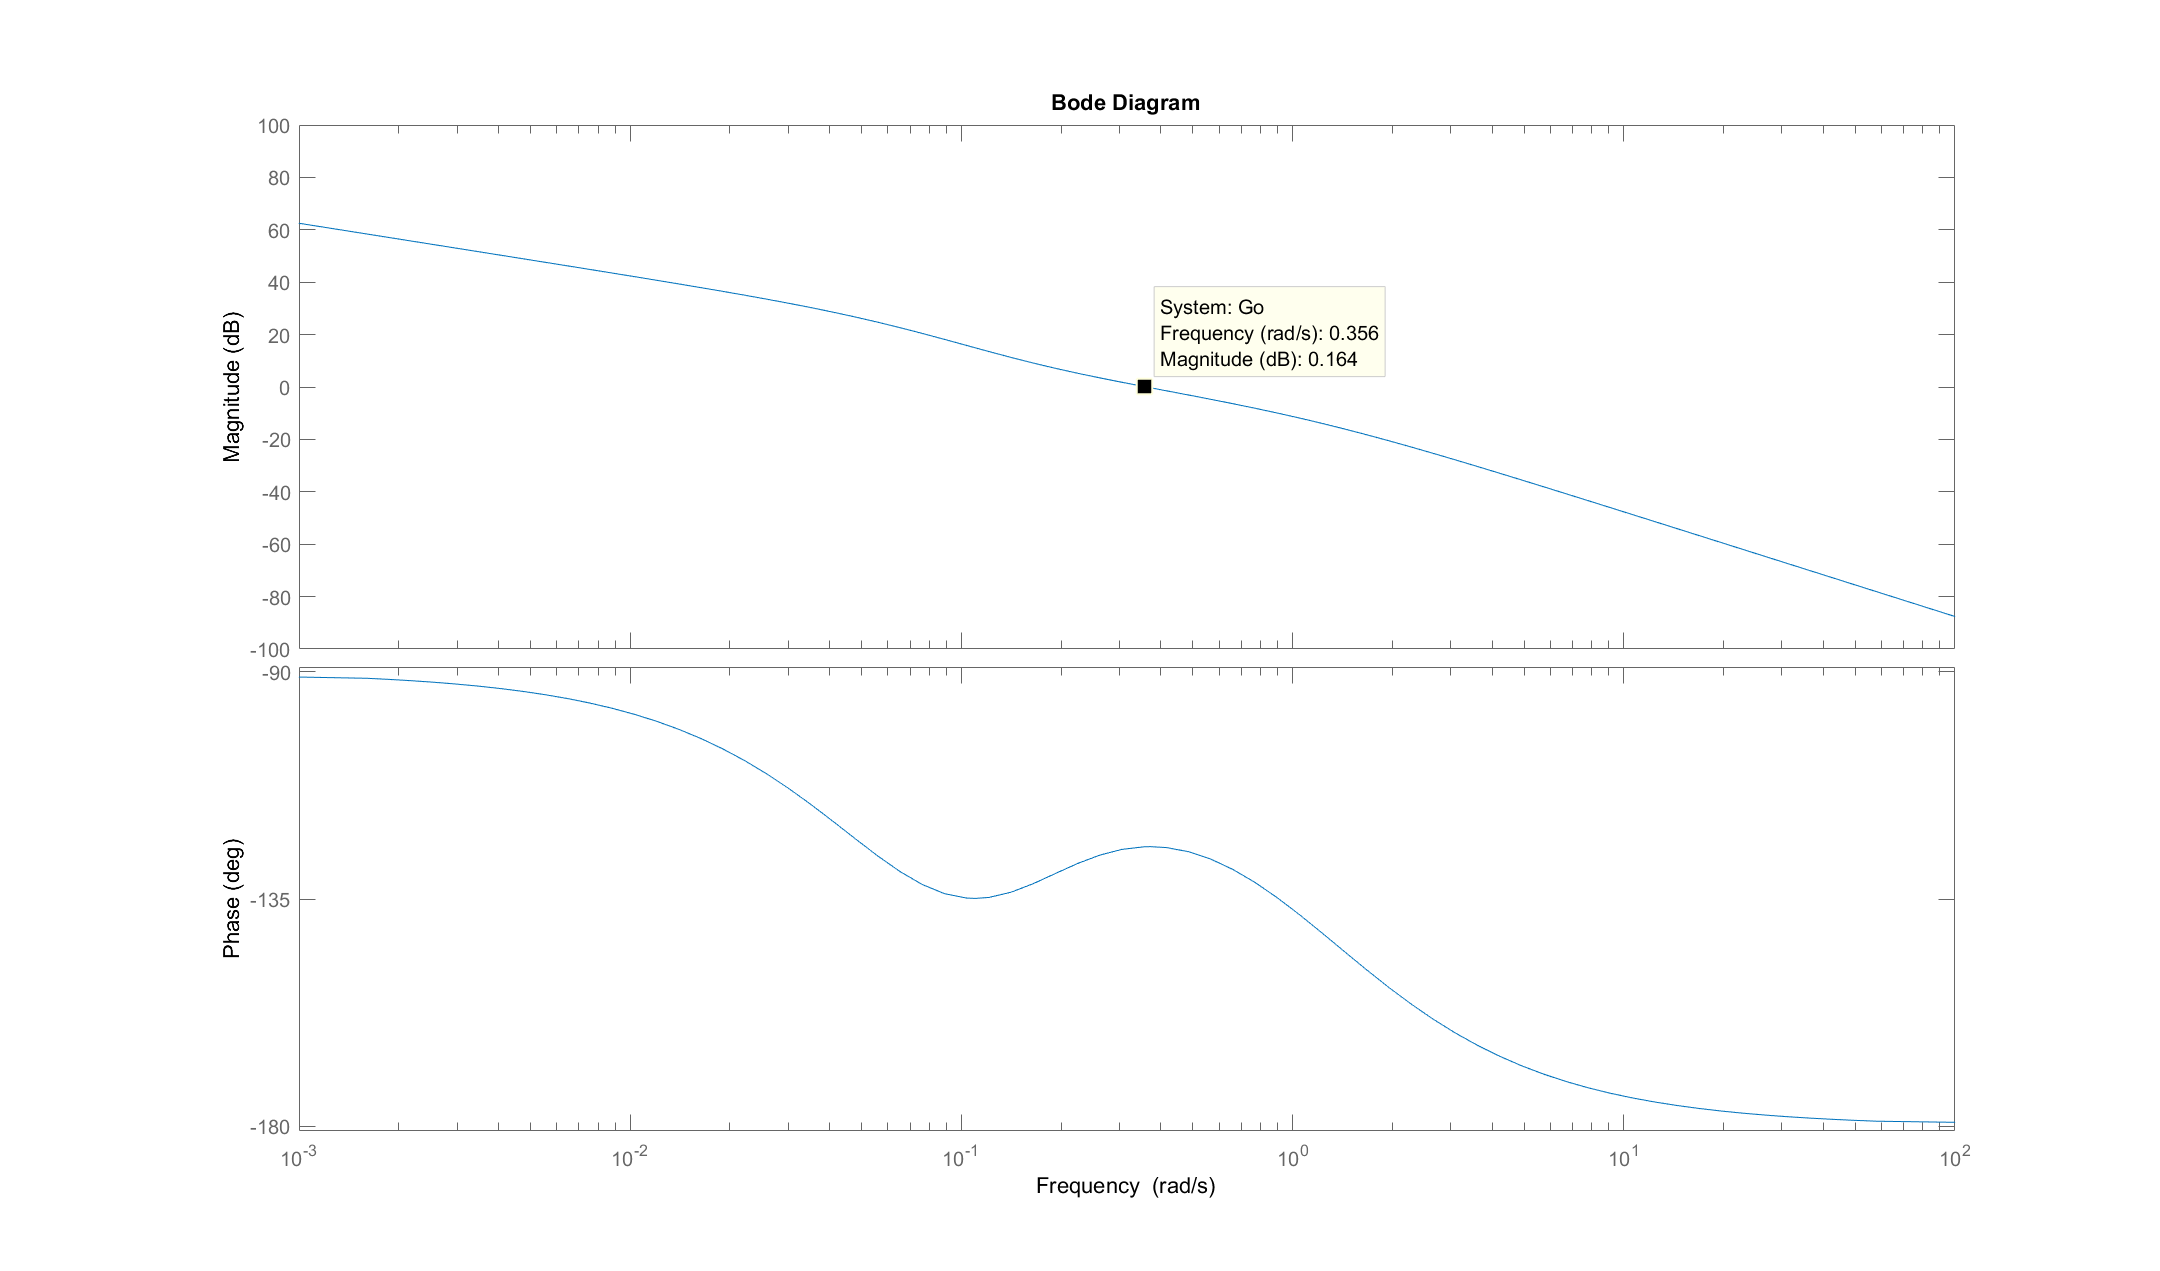
\includegraphics[width=\textwidth]{../Code/images/crossover.png}
    \end{figure}
    This is confirmed by the MatLab command \textit{allmargin(Go)} which gives
    $\omega_c = 0.343 \text{rad/s}$.
}
%%%%%% Part 2 %%%%%%%
\q %7
{
    A ZOH block is placed after the controller. What is the effect?
}
{
    The effect of the system for different ZOH times is shown below.
    \begin{figure}[H]
        \centering
        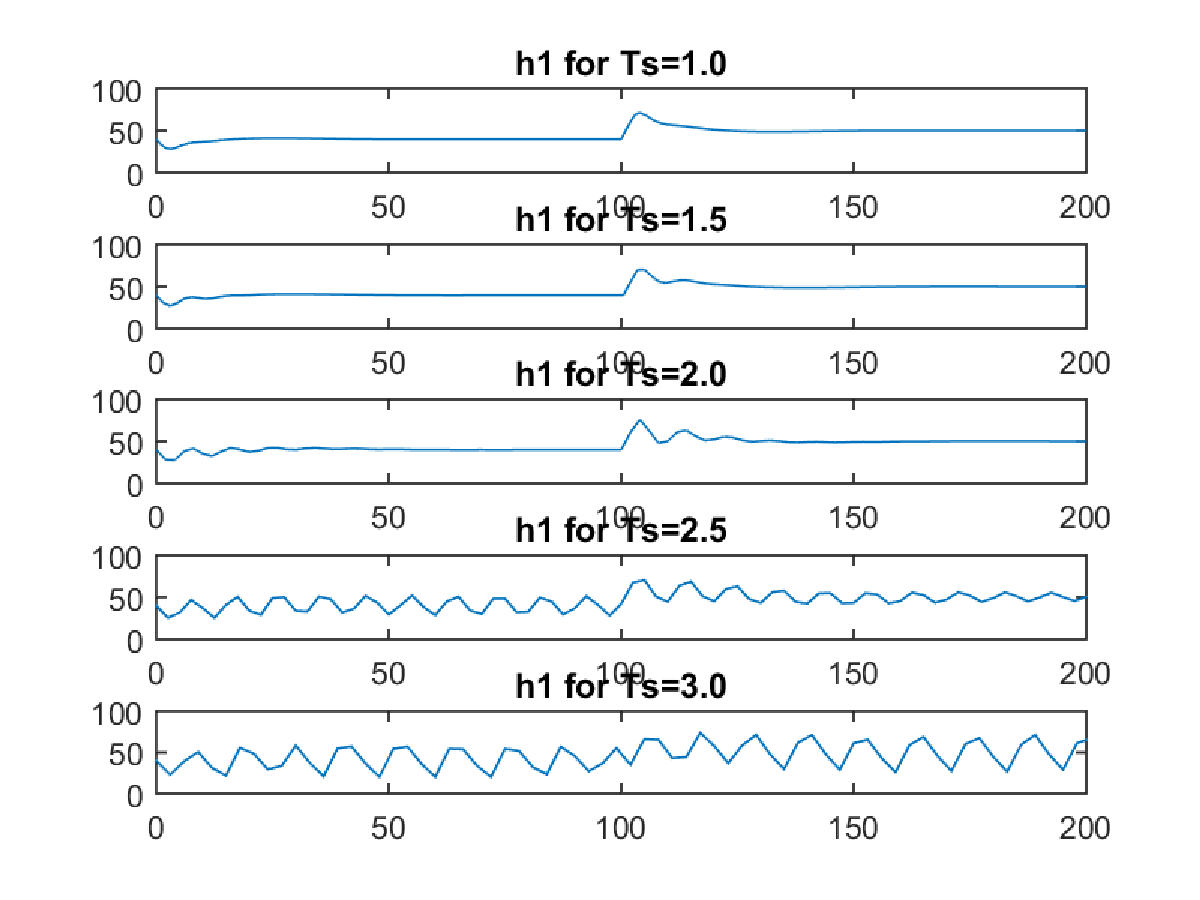
\includegraphics[width=\textwidth]{../Code/images/h1_samplings.png}
        \caption{Upper tank level for different sampling times.}
    \end{figure}
    \begin{figure}[H]
        \centering
        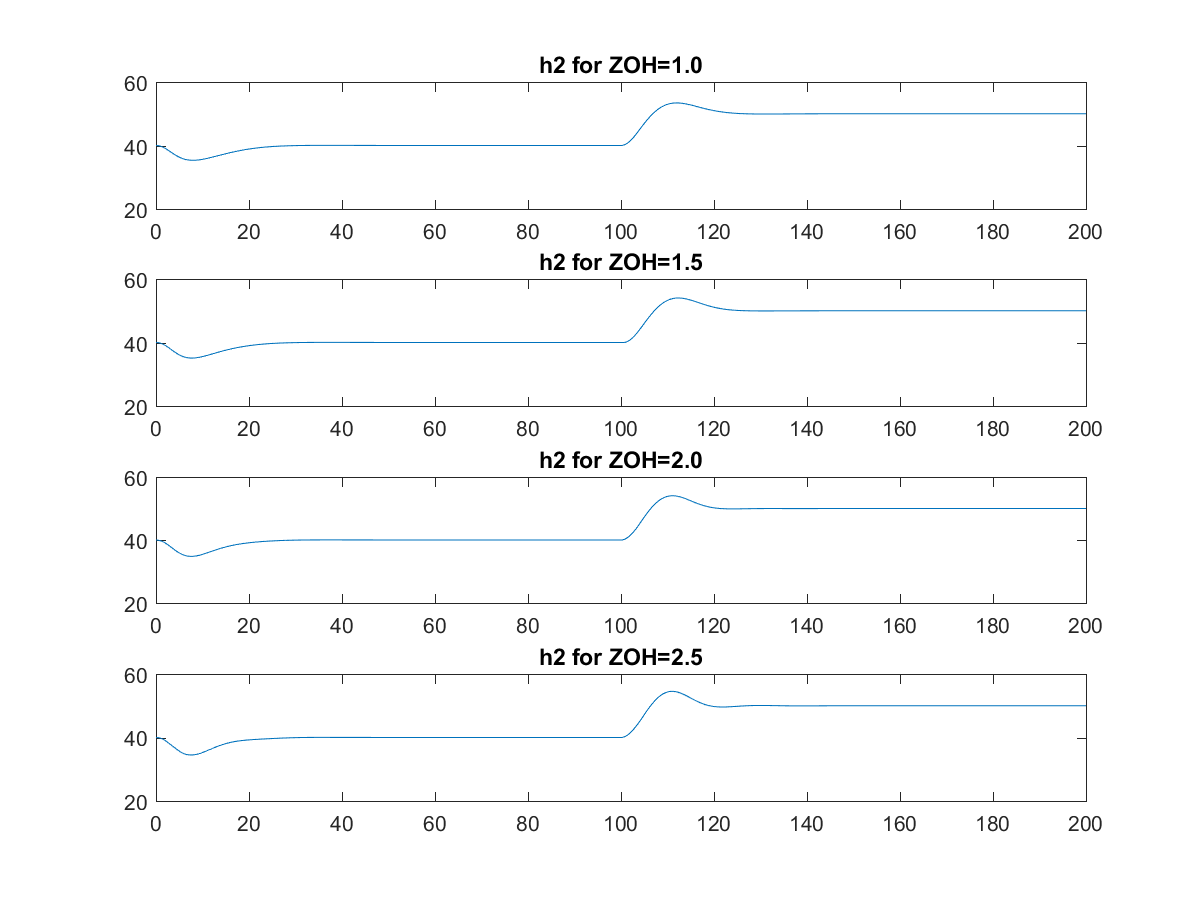
\includegraphics[width=\textwidth]{../Code/images/h2_samplings.png}
        \caption{Lower tank level for different sampling times.}
    \end{figure}
    \begin{figure}[H]
        \centering
        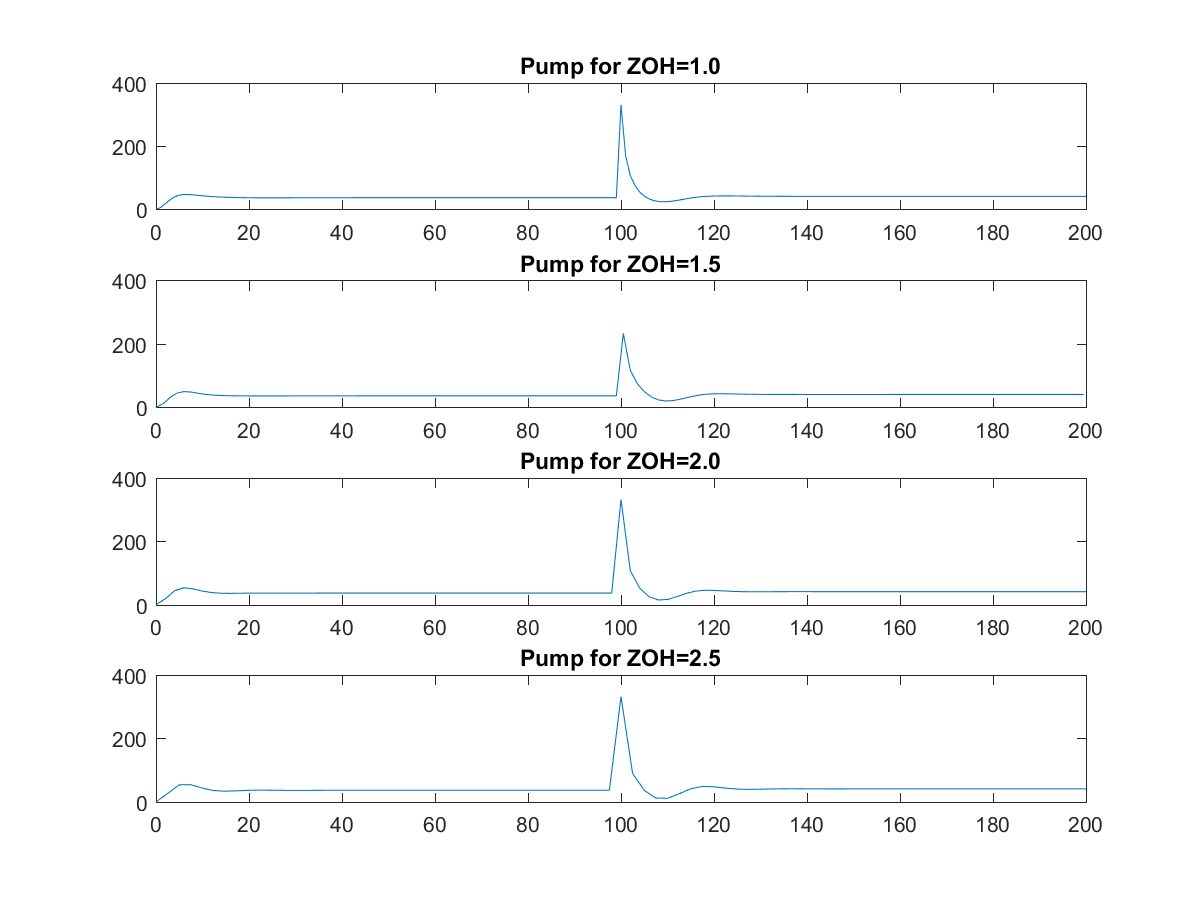
\includegraphics[width=\textwidth]{../Code/images/pump_samplings.png}
        \caption{Pump input for different sampling times.}
    \end{figure}
    From the figures it can be seen that the stabilility and performance of the
    system decreases with higher samplnig time. For a sampling time of about 1
    second, the system is stable and the performance is smooth. At 3 second
    sampling time, it is oscillating and is on the verge of becoming unstable.
}
\q %8
{
    Discretize the continuous controller into state space form. Replace the
    simulink controller block with this new discrete controller. What differences
    can be seen? 
}
{
    The performance of the sampled system is displayed below.
    \begin{figure}[H]
        \centering
        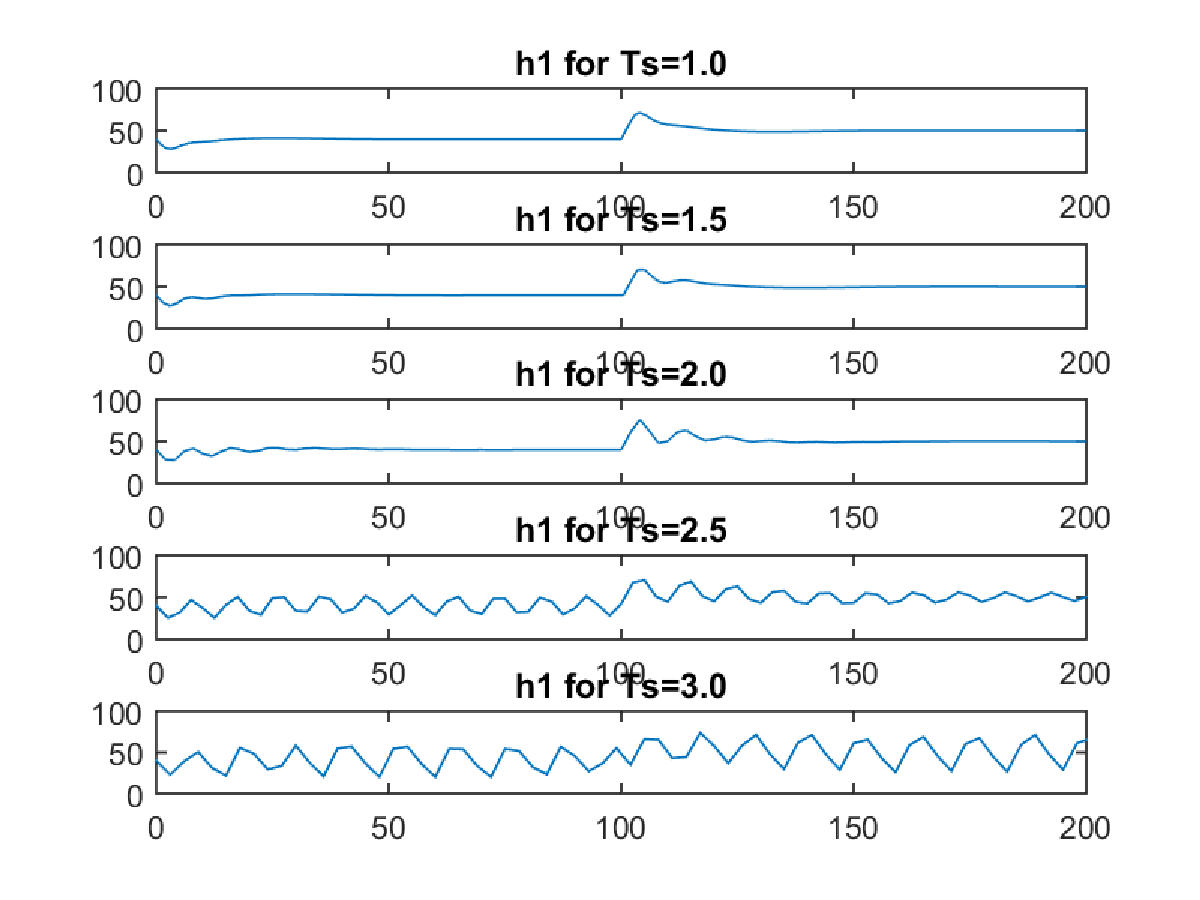
\includegraphics[width=\textwidth]{../Code/images/h1_samplings_ss.png}
        \caption{Upper tank level for different sampling times.}
    \end{figure}
    \begin{figure}[H]
        \centering
        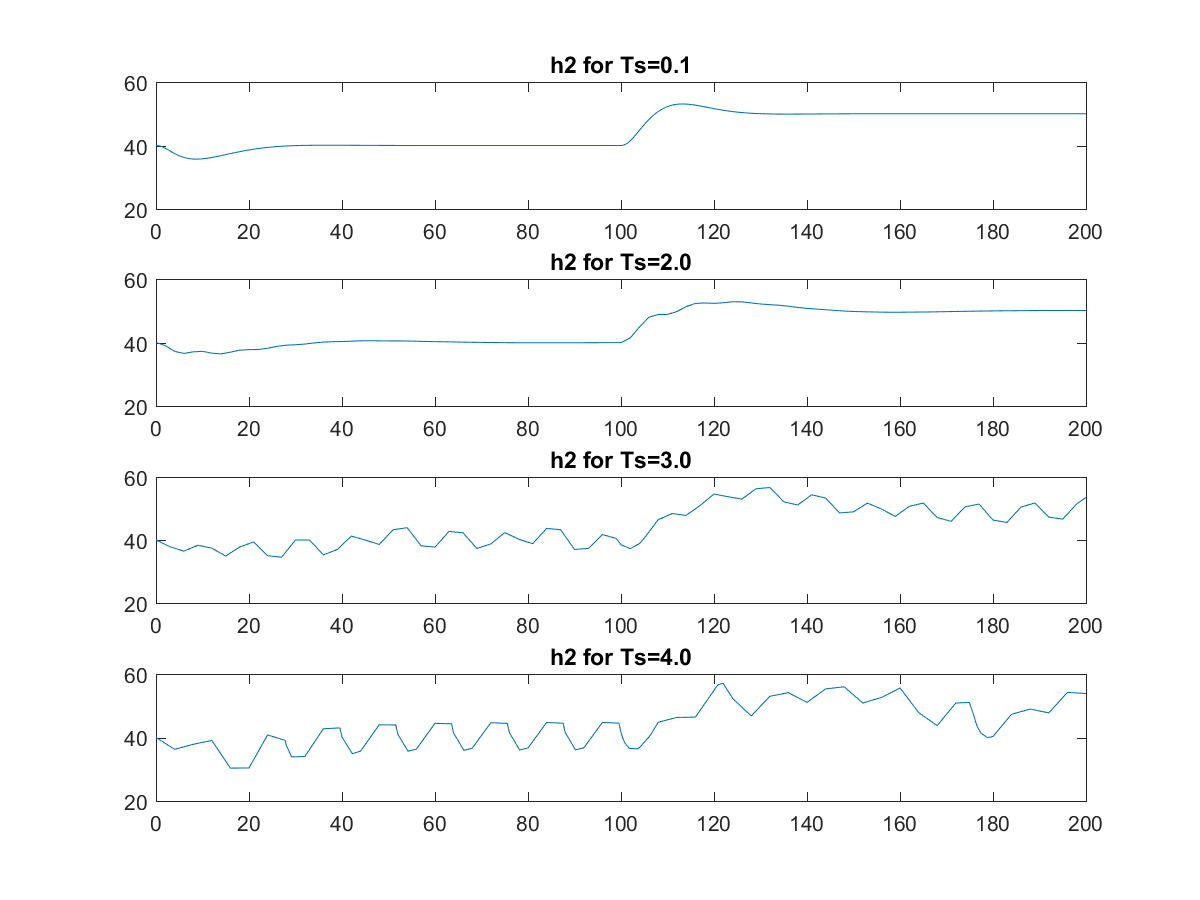
\includegraphics[width=\textwidth]{../Code/images/h2_samplings_ss.png}
        \caption{Lower tank level for different sampling times.}
    \end{figure}
    \begin{figure}[H]
        \centering
        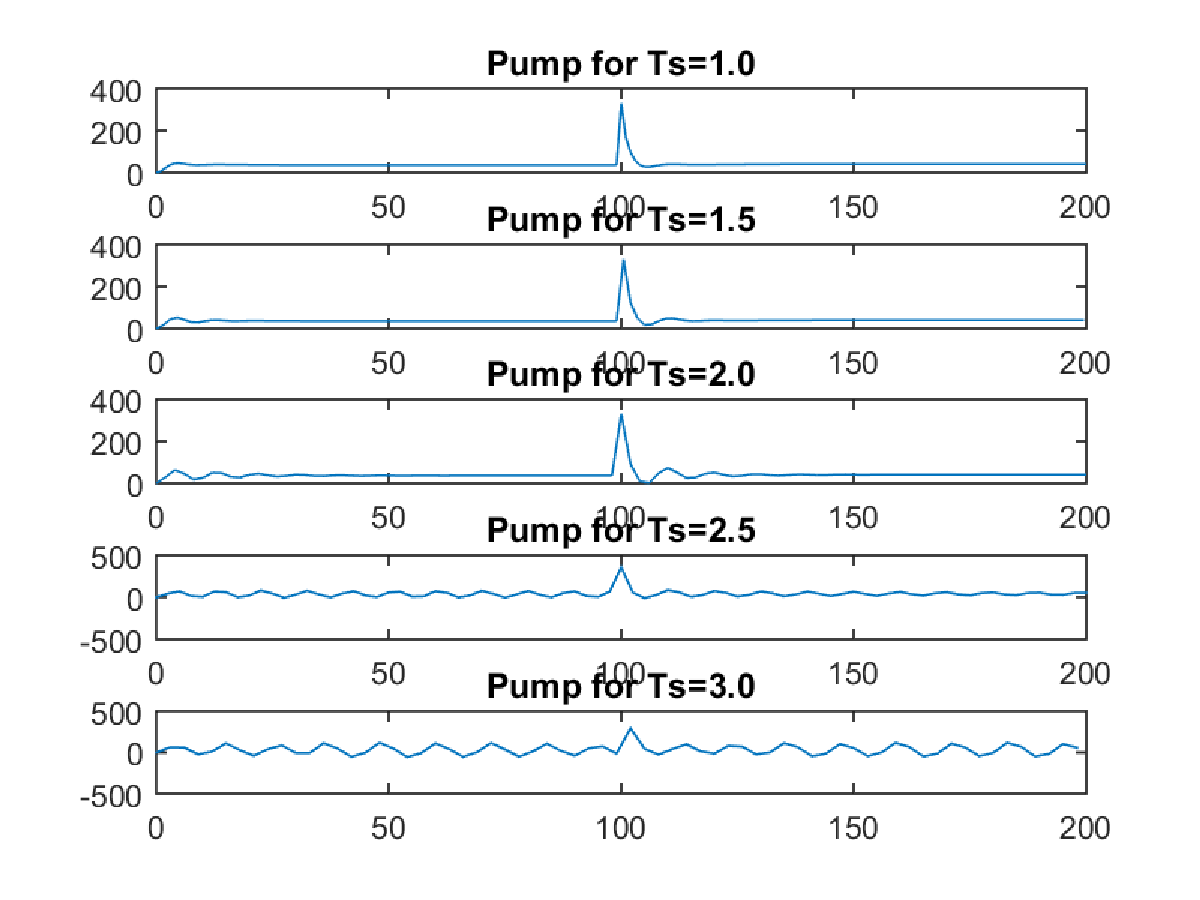
\includegraphics[width=\textwidth]{../Code/images/pump_samplings_ss.png}
        \caption{Pump input for different sampling times.}
    \end{figure}

    Comparison shows that ZOH method yields overall better results. This may be
    due to that the continuous system on which the ZOH method is based is more
    precise.
}

\q %9
{
     What sampling time should be chosen?
}
{
    The crossover frequency of the open-loop system is $\omega_c = 0.36 
    \text{rad/s}$. The thumbrule states that the sampling frequency should be
    approximately $20\omega_c  = 7.2 rad/s$. This gives a samplingtime of
    $\frac{2\pi}{20\omega_c} = 0.87 $ seconds
}
\q %10
{
    How long can the samplingtime be without affecting the performance?
}
{
    From question 8 it can be seen that the system is performing well up until a
    sampling time of about 2 seconds which is a little more than twice as fast
    as the rule of thumb in question 9.
}

\q %11
{
    Simulate system with samplingtime at 4 seconds and estimate the control
    performance.
}
{
    As can be seen below, the system is asymptotically stable but oscillating
    heavily. Controller performance is not good.
    \begin{figure}[H]
        \centering
        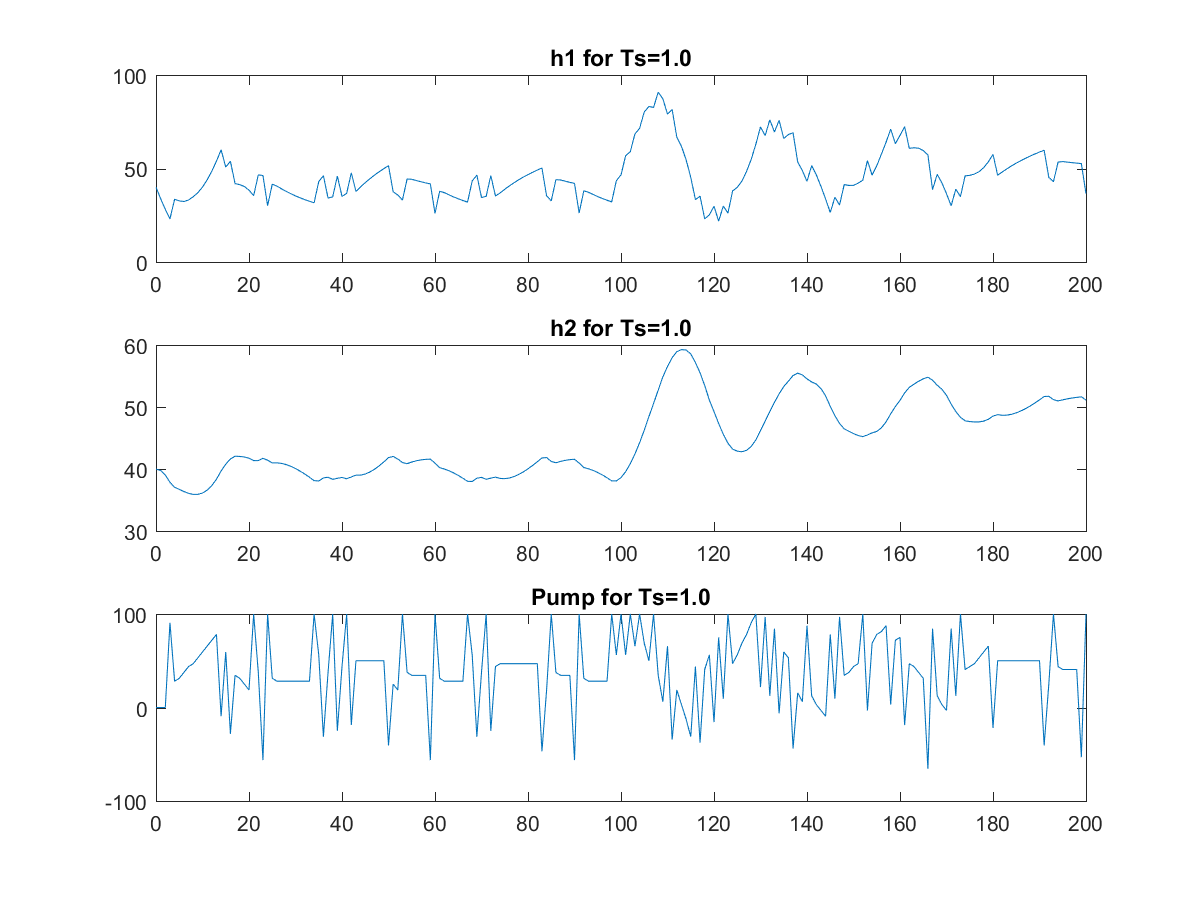
\includegraphics[width=\textwidth]{../Code/images/4s_samplings.png}
    \end{figure}
}
\q %12
{
    Sample G, make Gd
}
{
    The coefficients are shown in the table below.
    \begin{table}[H]
        \centering
            \begin{tabular}{|c|c|}
            \hline 
            $a_1$ &  0.092 \\
            \hline
            $a_2$ & 0.074 \\
            \hline
            $b_1$ & -1.4 \\
            \hline
            $b_2$ & 0.52 \\
            \hline
            \end{tabular}
    \end{table}
}
\q %13
{
    Where should discrete poles be placed?
}
{
    For a stable discrete system, the poles should be located within the unit
    circle.
}
\q %14
{
    What are the poles corresponding to the continuous poles in the discrete
    case? Also, what is the pole polynomial for discrete?
}
{
    After removing pole/zero pairs that cancel out, the continuous system
    contains one double pole on the real axis at -0.5 and a pair of complex
    conjugate poles at $0.16\pm0.12i$. Remapping to discrete poles $z_i=e^{T_s
    p_i}$ where $T_s$ is the sampling time of 4 s, the poles in the discrete
    case are as displayed in the table below.
    \begin{table}[htpb]
        \centering
        \begin{tabular}{c|c}
            Poles & Comment \\
            \hline
            $0.13$ & Real, double \\
            \hline
            $0.47+0.24i$ & Complex \\
            \hline
            $0.47-0.24i$ & Complex \\
        \end{tabular}
    \end{table}
    Using matlabs \textit{poly} command, the pole polynomial becomes
    \begin{equation}
        0=z^4 - 1.2z^3 + 0.55z^2 - 0.094z + 0.0051
    \end{equation}
}
\q %15
{
    Show that the closed system equations turn into the equation system.
}
{
    For the system
    \begin{equation}
        \label{eq:G}
        G= \frac{a_1z + a_2}{z^2 + b_1z + b_2}
    \end{equation}
    and the desired regulator
    \begin{equation}
        \label{eq:F}
        F = \frac{c_0z^2 + c_1 z + c_2}{(z-1)(z + r)}.
    \end{equation}
    The closed loop system has the equation
    \begin{equation}
        \label{eq:Gc}
       \frac{FG}{1+FG}.
    \end{equation}
    Using \ref{eq:F}, \ref{eq:G} and \ref{eq:Gc} and looking only at the
    denominator yields the pole equation
    \begin{equation}
        \label{eq:roots}
        z^4 + (b_1 + r -1 + c_0a_1)z^3 + (b_2 + b_13 - b_1 - r + c_0a_2 +
        c_1a_1)z^2 + (b_2r - b_2 -b_1r + c_1a_2 - c_2a_1)z + c_2a_2 -rb_2 = 0.
    \end{equation}
    Setting \ref{eq:roots} equal to the pole polynomial calculated in task 14
    and solving for each power of $z$ separately yields the equation system in
    task 15.
}

\q %16
{
	Solve the equation to get a discrete controller.
}
{
	Solving the linear equation system gives \\
	\begin{equation}
		F_d = \frac{20.4 - 35.7*z^{-1} + 15.7*z^{-2}}{1 - 1.20z^{-1} + 0.197z^{-2}}
	\end{equation}
    %Det är svårt att jämföra bilder på Gdc och Gc pzmap då den ena visar
    %kontinuerliga poler och den andra diskreta. Visar värden istället.
    The two systems poles after minimal realization is as follows:
    \begin{table}[H]
        \centering
         \begin{tabular}{|c|c|c|}
         \hline 
         $Poles$ &  $G_c$ &  $G_{dc}$\\
         \hline
         1  & 0.61 $\pm$ 0i  &    0.61 $\pm$ 0i \\ 
         %Repeat ad absurdum. Väntar tills vi är säkra på att det är rätt
         \hline
         2  & 0.85 $\pm$ 0.10i & 0.85 $\pm$ 0.10i\\
         \hline
         3  & - & 0.92 $\pm$ 0i\\
         \hline
         \end{tabular}
    \end{table}
    Four poles are exactly equal whilst $G_{dc}$ has an additional real pole.
    This is since AAAAAAAAAA.  We thus conclude that their performance are
    equal.
    
}

\q %17
{
	Simulate the system and compare with question 11.
}
{
	The system from question 11
    \begin{figure}[H]
        \centering
        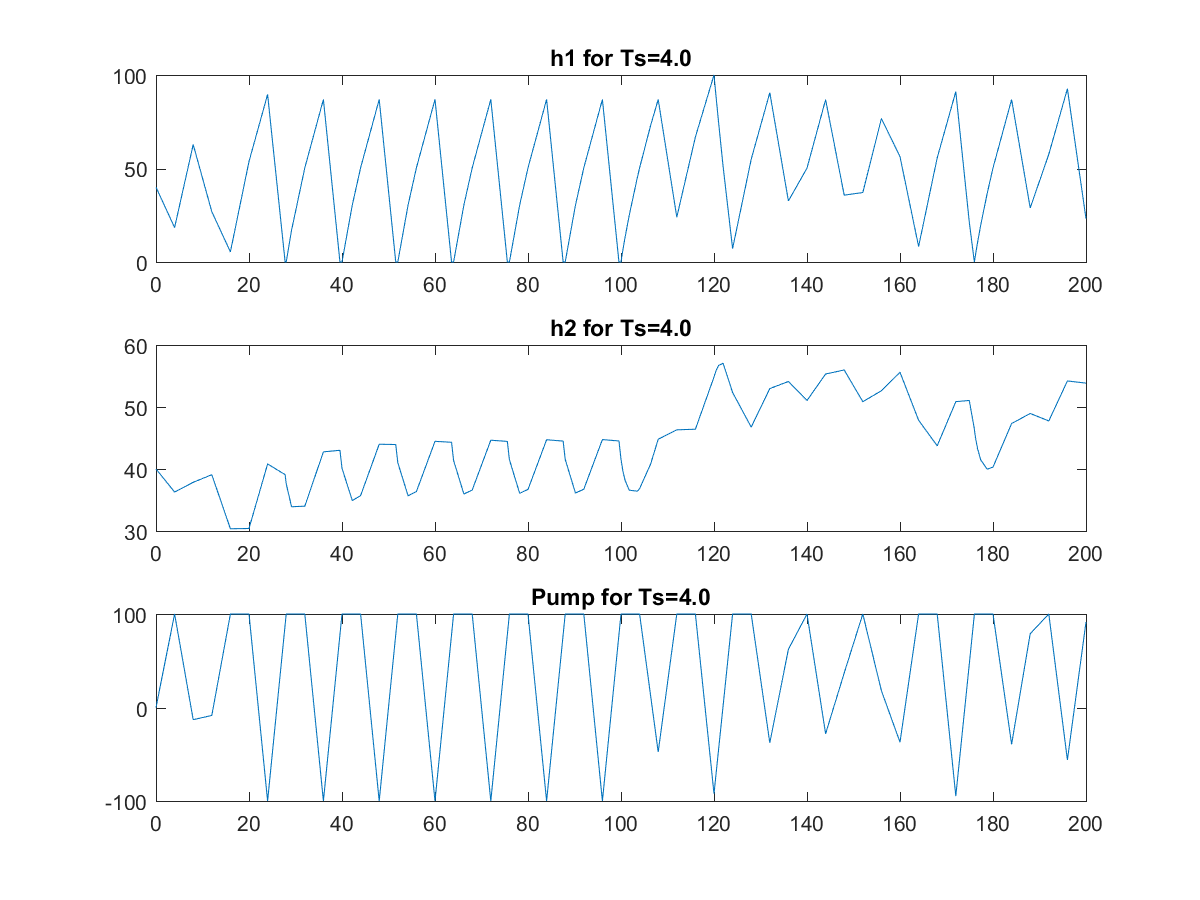
\includegraphics[width=\textwidth]{../Code/images/all_q11.png}
    \end{figure}
    The current system
    \begin{figure}[H]
        \centering
        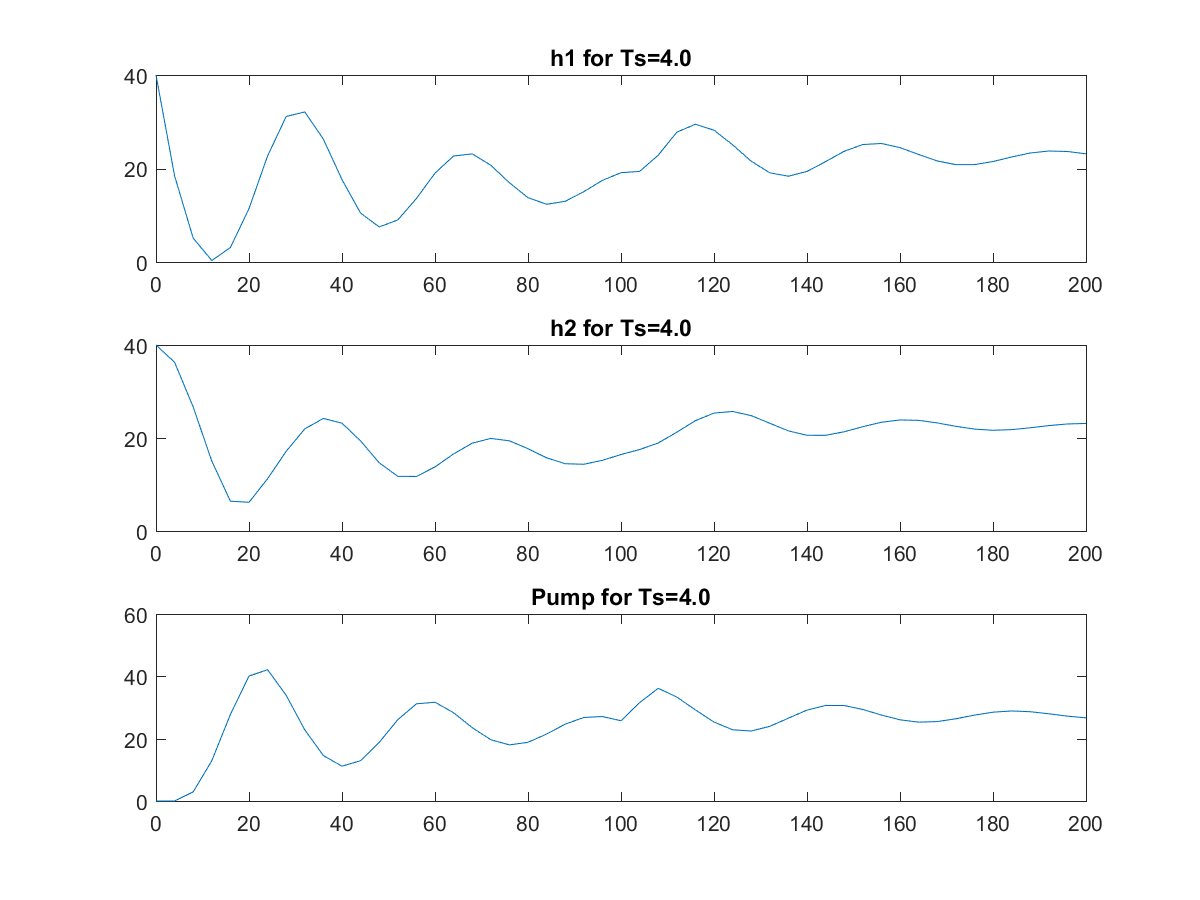
\includegraphics[width=\textwidth]{../Code/images/all_q17.png}
    \end{figure}

	Here a great improvement can be seen.
}

\q %18
{
	With a signal between 0 and 100 and a 10 bit A/D converter, what is the quantization level?
}
{
	$ quantization = \frac{0-100}{2^{10}} = 9.77*10^{-4}$
}
\q % 19
{
	Attempt to connect a quantization block to a saturation block
}
{
    \begin{figure}[H]
        \centering
        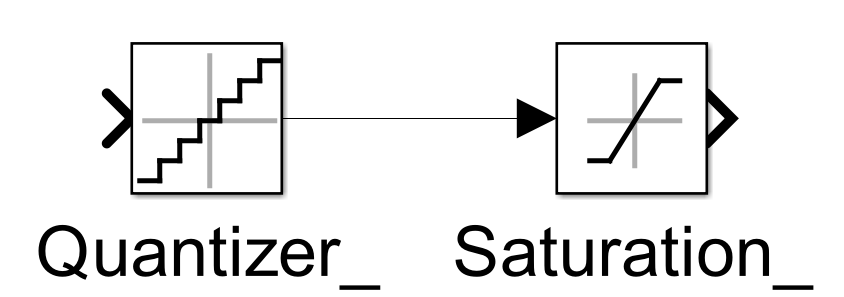
\includegraphics[width=\textwidth]{../images/q19.png}
    \end{figure}
    Done!
}

\q % 20
{
	Connect above model before and after the discrete designed controller. Simulate for different values of quantization and determine at which level the control performance starts to degrade.
}
{
	The system was tested with multiple quantizationlevels determined by $\frac{100-(-100)}{s^n} = quantization$
	\begin{figure}[H]
        \centering
        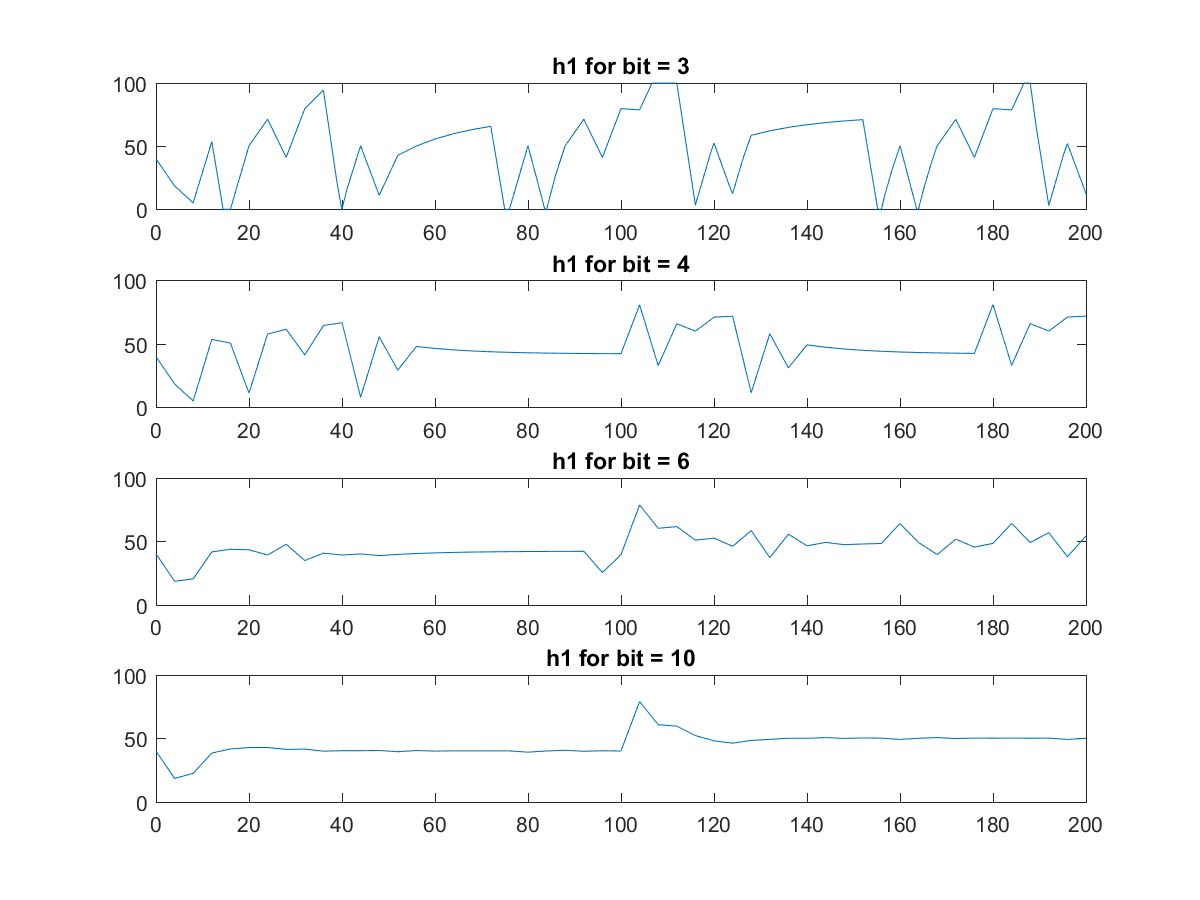
\includegraphics[width=\textwidth]{../Code/images/h1_quant_samplings.png}
    	\end{figure}
        \begin{figure}[H]
        \centering
        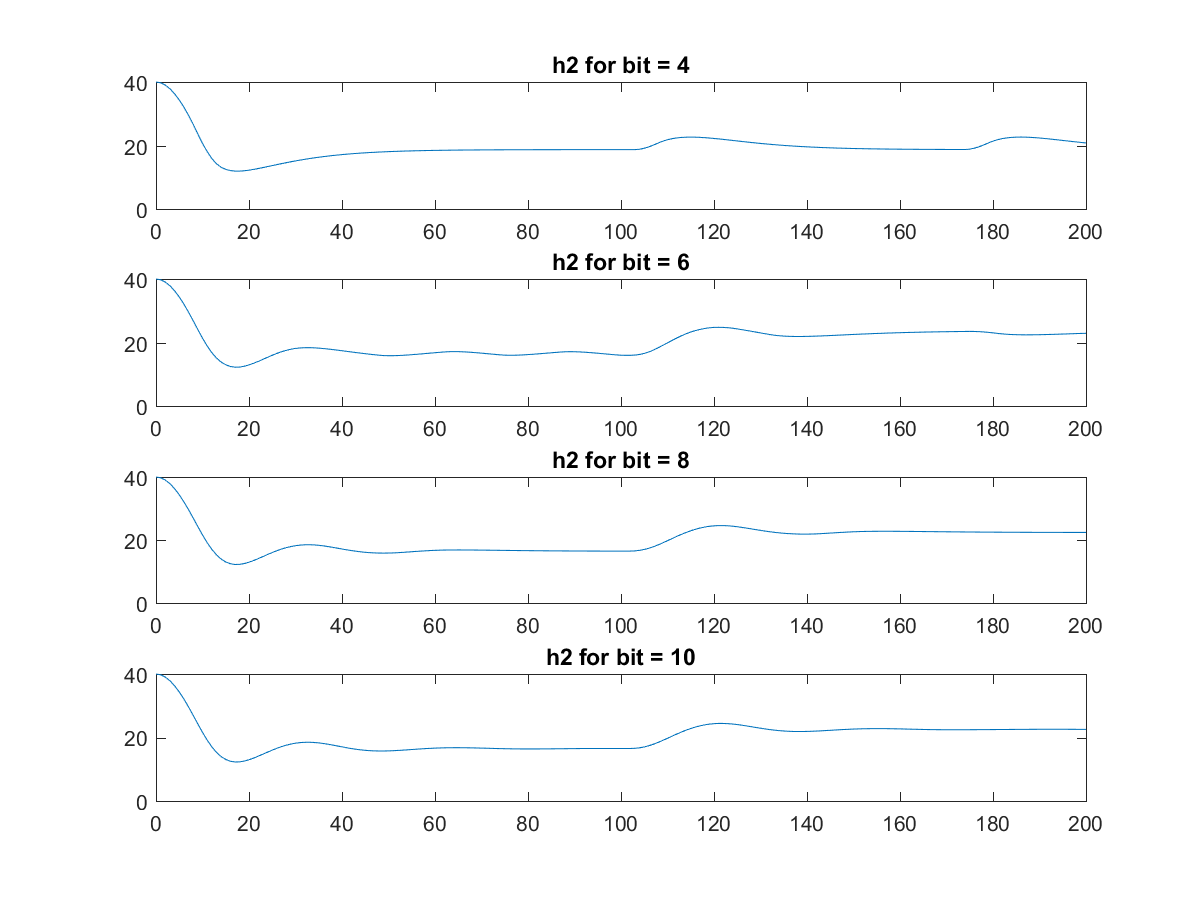
\includegraphics[width=\textwidth]{../Code/images/h2_quant_samplings.png}
    	\end{figure}
	\begin{figure}[H]
        \centering
        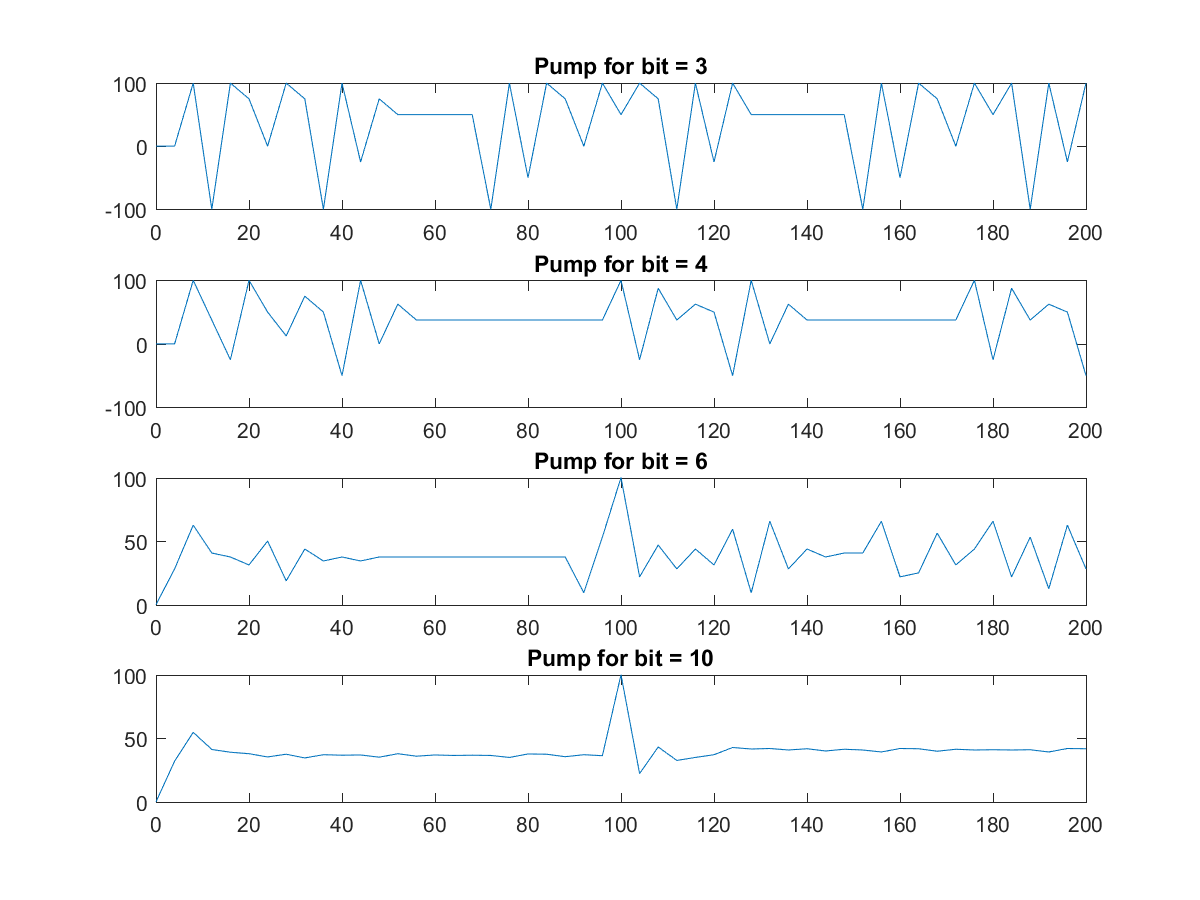
\includegraphics[width=\textwidth]{../Code/images/pump_quant_samplings.png}
   	\end{figure}
   	
   	Exactly when the system performance starts to degrade is subjective, but it is clear that when the system goes below a 4-bit A{\textbackslash}D converter the performance is seriously hampered.
}
\end{document}
